\documentclass[12pt]{report}
\usepackage{amsmath,amsthm,amsfonts,amscd,amssymb,eucal,latexsym,fullpage,fancyhdr,lastpage}
\usepackage{tikz}
\usetikzlibrary{plotmarks}
\usetikzlibrary{shapes.geometric}
\usetikzlibrary{positioning}
\usetikzlibrary{decorations.pathreplacing}
\renewcommand{\baselinestretch}{1}
\setlength{\textwidth}{16.5cm}
\setlength{\oddsidemargin}{0cm}
\setlength{\evensidemargin}{0cm}
\pagestyle{fancy}
\fancyhf{}
\renewcommand{\headrulewidth}{0pt}
\cfoot{\thepage \ of \pageref{LastPage}}

%%%%%%%%%%%%%%%%%%%%%%%%%%%%%%%%%%%%%%%%%%%%%%%%%%%%%%%%%%%%%%%%%%%%
\begin{document}
%%%%%%%%%%%%%%%%%%%%%%%%%%%%%%%%%%%%%%%%%%%%%%%%%%%%%%%%%%%%%%%%%%%%

\vspace*{0.25in}
\begin{center}
%{\sc Report to the Research Assessment Committee}\\[10mm]
{\Large\bf
Limit Order Book Imbalance}\\[2mm]
{\large Anton Rubisov}\\%[-1mm]
%{\footnotesize\it anton.rubisov@mail.utoronto.ca}\\[2mm]
%The Space Robotics Group\\
%Institute for Aerospace Studies\\
%University of Toronto\\
%4925 Dufferin Street\\
%Toronto, Ontario, Canada M3H 5T6\\[3mm]
{\small 2014.07.17}
\end{center}

\paragraph{Research Direction} \mbox{} \\

To predict future stock price movement based on current price and order book imbalance. That is,
$$ \dot{p} = f(p,I)$$

\paragraph{Framework} \mbox{} \\

Limit order book imbalance is a ratio of limit order volumes between the bid and ask side, and can be calculated for example as $I(t) = \dfrac{V_b(t) - V_a(t)}{V_b(t) + V_a(t)} \in [-1,1]$.
\begin{itemize}
\item We bin the bid/ask volume imbalances in the Limit Order Book into $K$ bins, each being dubbed a ``regime'' of the limit order book. 
\item $Z_t$ is a continuous-time Markov chain that tracks which regime we're in. $Z_t$ takes values in $\{1, \dots , K\}$, and has an infinitesimal generator matrix $G$.
\item Conditional on being in some regime $k$, the arrival of buy and sell market orders follow independent Poisson processes with intensities $\lambda^{\pm}_k$.
\end{itemize}

We have observations of arrivals of buy/sell market orders and of regime switches occurring, all of which are timestamped. Pictorially, a timeline might look like: \\

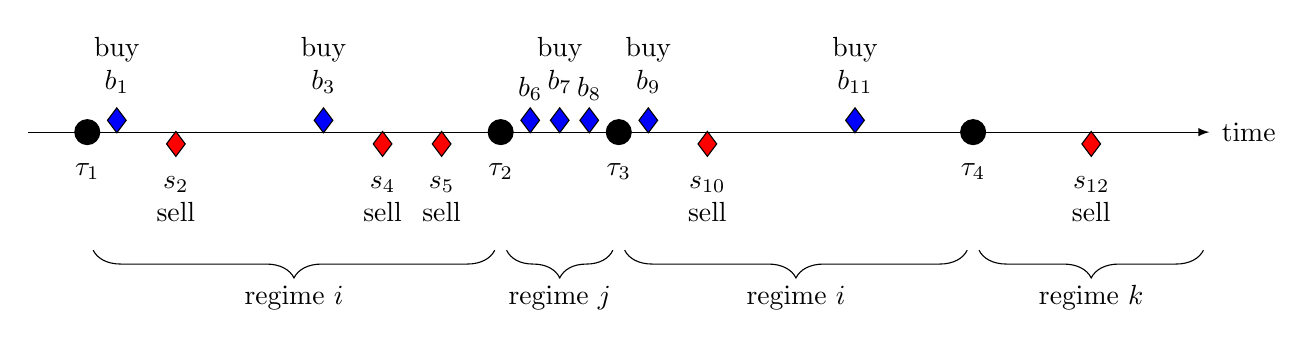
\begin{tikzpicture}[scale=1.5]
	[triangle/.style = {fill=blue!20, regular polygon, regular polygon sides=3 },
	border rotated/.style = {shape border rotate=180}]
	
	
    \draw [>=latex,->] (0,0) -- (10,0) node[draw=none,fill=none,shift=(right:0.5)] {time};
    \draw[mark options={fill=black}, mark size=+3pt] plot[mark=*] coordinates {(.5,0)} node[shift=(down:0.5), align=center] {$\tau_1$};
    \draw[mark options={fill=black}, mark size=+3pt] plot[mark=*] coordinates {(4,0)} node[shift=(down:0.5), align=center] {$\tau_2$};
    \draw[mark options={fill=black}, mark size=+3pt] plot[mark=*] coordinates {(5,0)} node[shift=(down:0.5), align=center] {$\tau_3$};
    \draw[mark options={fill=black}, mark size=+3pt] plot[mark=*] coordinates {(8,0)} node[shift=(down:0.5), align=center] {$\tau_4$};
    
    
	\draw[mark options={fill=blue}, mark size =+3pt, shift=(up:0.1)] plot[mark=diamond*] coordinates {(.75,0)} node[shift=(up:0.7), align=center] {buy \\ $b_1$};
	\draw[mark options={fill=red}, mark size =+3pt, shift=(down:0.1)] plot[mark=diamond*] coordinates {(1.25,0)} node[shift=(down:0.7), align=center] {$s_2$ \\ sell};
	\draw[mark options={fill=blue}, mark size =+3pt, shift=(up:0.1)] plot[mark=diamond*] coordinates {(2.5,0)} node[shift=(up:0.7), align=center] {buy \\ $b_3$};
	\draw[mark options={fill=red}, mark size =+3pt, shift=(down:0.1)] plot[mark=diamond*] coordinates {(3,0)} node[shift=(down:0.7), align=center] {$s_4$ \\ sell};
	\draw[mark options={fill=red}, mark size =+3pt, shift=(down:0.1)] plot[mark=diamond*] coordinates {(3.5,0)} node[shift=(down:0.7), align=center] {$s_5$ \\ sell};

%%% REGIME SWITCH
	
	\draw[mark options={fill=blue}, mark size =+3pt, shift=(up:0.1)] plot[mark=diamond*] coordinates {(4.25,0)} node[shift=(up:0.4), align=center] {$b_6$};
	\draw[mark options={fill=blue}, mark size =+3pt, shift=(up:0.1)] plot[mark=diamond*] coordinates {(4.50,0)} node[shift=(up:0.7), align=center]
{buy \\ $b_7$};
	\draw[mark options={fill=blue}, mark size =+3pt, shift=(up:0.1)] plot[mark=diamond*] coordinates {(4.75,0)} node[shift=(up:0.4), align=center] {$b_8$};
	
%%% REGIME SWITCH

	\draw[mark options={fill=blue}, mark size =+3pt, shift=(up:0.1)] plot[mark=diamond*] coordinates {(5.25,0)} node[shift=(up:0.7), align=center] {buy \\ $b_9$};
	\draw[mark options={fill=red}, mark size =+3pt, shift=(down:0.1)] plot[mark=diamond*] coordinates {(5.75,0)} node[shift=(down:0.7), align=center] {$s_{10}$ \\ sell};
	\draw[mark options={fill=blue}, mark size =+3pt, shift=(up:0.1)] plot[mark=diamond*] coordinates {(7,0)} node[shift=(up:0.7), align=center] {buy \\ $b_{11}$};
	
%%% REGIME SWITCH

	\draw[mark options={fill=red}, mark size =+3pt, shift=(down:0.1)] plot[mark=diamond*] coordinates {(9,0)} node[shift=(down:0.7), align=center] {$s_{12}$ \\ sell};
	
%%% BRACES
	
	\draw [decorate, decoration = {brace, amplitude = 10pt, mirror}]
	(0.55,-1) -- (3.95,-1) node [black, midway, yshift = -0.6cm] {regime $i$};
	\draw [decorate, decoration = {brace, amplitude = 10pt, mirror}]
	(4.05,-1) -- (4.95,-1) node [black, midway, yshift = -0.6cm] {regime $j$}; 
	\draw [decorate, decoration = {brace, amplitude = 10pt, mirror}]
	(5.05,-1) -- (7.95,-1) node [black, midway, yshift = -0.6cm] {regime $i$}; 
	\draw [decorate, decoration = {brace, amplitude = 10pt, mirror}]
	(8.05,-1) -- (9.95,-1) node [black, midway, yshift = -0.6cm] {regime $k$}; 

\end{tikzpicture}

\paragraph{Maximum Likelihood Estimation of $G$} \mbox{} \\

Let $G$ be the generator matrix for $Z_t$, so $G = \{ q_{ij} \} \in \mathbb{R}^{K \times K}$ where $q_{ij}$ are the transition rates from regime $i$ to regime $j$ for $i\neq j$, and $q_{ii} = - \sum\limits_{j \neq i} q_{ij}$ so that the rows of $G$ sum to 0. 

When $Z_t$ enters regime $i$, the amount of time it spends in regime $i$ is exponentially distributed with rate $v_i = \sum\limits_{j \neq i} q_{ij}$, and when it leaves regime $i$ it will to go regime $j$ with probability $p_{ij} = \dfrac{q_{ij}}{v_i}$. 

From our observations we want to estimate the components of $G$. The holding time in a given regime $i$ is exponentially distributed with pdf $f(t;v_i) = v_i e^{-v_i t}$. For the fictional events in the timeline above, the likelihood function (allowing for repetition of terms) would therefore be:

\begin{align*}
\mathcal{L}(G) &= (v_{i} e^{-v_{i}(\tau_2 - \tau_1)} p_{ij}) (v_{j} e^{-v_{j}(\tau_3 - \tau_2)} p_{ji}) (v_{i} e^{-v_{i}(\tau_4 - \tau_3)} p_{ik}) \dots \\
&= \prod\limits_{i=1}^{K} \prod\limits_{i \neq j} (v_{i}p_{ij})^{N_{ij}(T)} e^{-v_{i}H_i(T)} \\
&= \prod\limits_{i=1}^{K} \prod\limits_{i \neq j} (q_{ij})^{N_{ij}(T)} e^{-v_{i}H_i(T)} \\
\intertext{where:}
N_{ij}(T) & \equiv \mbox{number of transitions from regime $i$ to $j$ up to time $T$} \\
H_{i}(T) & \equiv \mbox{holding time in regime $i$ up to time $T$} \\
\intertext{So that the log-likelihood becomes:} 
\ln \mathcal{L}(G) & = \sum\limits_{i=1}^{K} \sum\limits_{i \neq j} \left[ N_{ij}(T) \ln(q_{ij}) - v_{i} H_i(T) \right] \\
&= \sum\limits_{i=1}^{K} \sum\limits_{i \neq j} \left[ N_{ij}(T) \ln(q_{ij}) - \left( \sum\limits_{i \neq k} q_{ik} H_i(T) \right) \right]
\end{align*}

To get a maximum likelihood estimate $\hat{q}_{ij}$ for transition rates and therefore the matrix $G$, we take the partial derivative of $\ln \mathcal{L}(G)$ and set it equal to zero:

$$\dfrac{\partial \ln \mathcal{L}(G)}{\partial q_{ij}} = \dfrac{N_{ij}(T)}{q_{ij}} - H_i(T) = 0$$
$$ \Rightarrow \hat{q}_{ij} = \dfrac{N_{ij}(T)}{H_i(T)}$$



\paragraph{Maximum Likelihood Estimation of $\lambda^{\pm}_k$} \mbox{} \\

Now we want to derive an estimate for the intensity of the Poisson process of market order arrivals conditional on being in some regime $k$. We'll look first at just the market buys for some regime $k$. In the above timeline, the market order buy arrival times are indexed by $b_i$. Since we're assuming that the arrival process is Poisson with the same intensity throughout trials, we can consider the inter-arrival time of events conditional on being in regime $k$. Then the MLE derivation follows just as for the CTMC:

\begin{align*}
\mathcal{L}(\lambda^{+}_k ; b_1, \dots, b_N) &= \prod\limits_{i=2}^{N} \lambda^{+}_k e^{-\lambda^{+}_k (b_{i} - b_{i-1})} \\
&= (\lambda^{+}_k)^{N^{+}_k(T)} e^{-\lambda^{+}_k H_k(T)} \\
\intertext{where:}
N^{+}_{k}(T) & \equiv \mbox{number of market order arrivals in regime $k$ up to time $T$} \\
H_{k}(T) & \equiv \mbox{holding time in regime $k$ up to time $T$} \\
\intertext{So that the log-likelihood becomes:} 
\ln \mathcal{L}(\lambda^{+}_k) & = N^{+}_k(T) \ln(\lambda^{+}_k) -\lambda^{+}_k H_k(T)
\intertext{And the ML estimate for $\hat{\lambda}^{+}_k$ is:} 
\dfrac{\partial \ln\mathcal{L} }{\partial \lambda^{+}_k} & = 
\dfrac{N^{+}_k(T)}{\lambda^{+}_k} - H_k(T) = 0
\end{align*}

$$ \Rightarrow \hat{\lambda}^{+}_k = \dfrac{N^{+}_k(T)}{H_k(T)}$$

%Now we want to derive an estimate for the intensity of the Poisson process of market order arrivals conditional on being in some regime $k$. We'll look first at just the market buys for some regime $k$ - call the random variable counting the number of market buys $X$. We want to estimate the intensity, $\lambda^{+}_k$, of the (Poisson) distribution of $X$, which is also the expected value of $X$ as well as its variance. Suppose we have $N$ observations of some fixed time interval of LOB activity in this regime, and the number of market buy events in each trial is $n_i$ for $i=1,\dots,N$.
%
%Assuming the distributions of each trial have the same intensity, the probability mass function gives us that for each $i$:
%
%$$P(X=n_i) = \frac{{\lambda^{+}_k}^{n_i} e^{-\lambda^{+}_k}}{n_i!}$$
%
%Since the trials are independent and identically distributed, the joint density function is:
%
%$$P(n_1, \dots, n_N | \lambda^{+}_k) = P(n_1 | \lambda^{+}_k) \times \dots \times P(n_N | \lambda^{+}_k)$$
%
%So the likelihood function is:
%$$\mathcal{L}(\lambda^{+}_k ; n_1, \dots, n_N) = \prod_{i=1}^{N} P(n_i | \lambda^{+}_k) = \prod_{i=1}^{N} \frac{{\lambda^{+}_k}^{n_i} e^{-\lambda^{+}_k}}{n_i!}$$
%
%Thus the log-likehood can be simplified (using logarithm and exponent identities) as:
%\begin{align*}
%\ln\mathcal{L} &= \ln \left(  \prod_{i=1}^{N} \frac{{\lambda^{+}_k}^{n_i} e^{-\lambda^{+}_k}}{n_i!} \right) \\
%&= \ln \left( \frac{{\lambda^{+}_k}^{\left(\sum_{i=1}^{N} n_i\right)} e^{-N\lambda^{+}_k}}{\prod_{i=1}^{N} n_i!} \right) \\
%&= \ln \left( {\lambda^{+}_k}^{\left(\sum_{i=1}^{N} n_i \right)} \right) - N\lambda^{+}_k - \sum_{i=1}^{N} \ln (n_i !)
%\end{align*}
%
%Now we can get a maximum likelihood estimate for $\lambda^{+}_k$ by taking the partial derivative of $\ln\mathcal{L}$ with respect to $\lambda^{+}_k$ and setting it equal to zero:
%
%$$ \frac{\partial \ln\mathcal{L} }{\partial \lambda^{+}_k} = 
%\dfrac{\sum\limits_{i=1}^{N} n_i}{\lambda^{+}_k} - N = 0$$
%$$\frac{\sum\limits_{i=1}^{N} n_i}{\lambda^{+}_k} = N$$
%$$\lambda^{+}_k = \frac{\sum\limits_{i=1}^{N} n_i}{N}$$

%%%%%%%%%%%%%%%%%%%%%%%%%%%%%%%%%%%%%%%%%%%%%%%%%%%%%%%%%%%%%%%%%%%%
\end{document}
%%%%%%%%%%%%%%%%%%%%%%%%%%%%%%%%%%%%%%%%%%%%%%%%%%%%%%%%%%%%%%%%%%%%